\chapter{Project Architecture}\label{ch:B}

\section{Hierarchy}
Since we have few roles in the web-site. We would like to show you hierarchy of users. (See Figure \ref{fig:Hierarchy}).

\begin{figure}[h!]
    \centering
    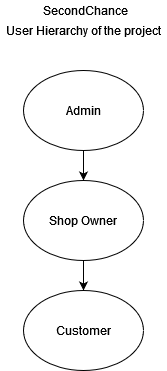
\includegraphics[scale=0.9]{figures/Hierarchy.png}
    \caption{User types}
    \label{fig:Hierarchy}
\end{figure}

\section{User case diagram}
This is a use case diagram, where you can understand how all system users work
In our case, there are three roles - Admin, Shop Owner, Customer.  Each of them has their own individual roles that are interconnected.  The admin can add or remove shop owners and stores.  And in turn, Shop Owners create or delete a store product, and they can also edit products.  For example, they can change the time of the auction.
Customers can purchase items only after registration. (See Figure \ref{fig:user-case}).

\begin{figure}[h!]
    \centering
    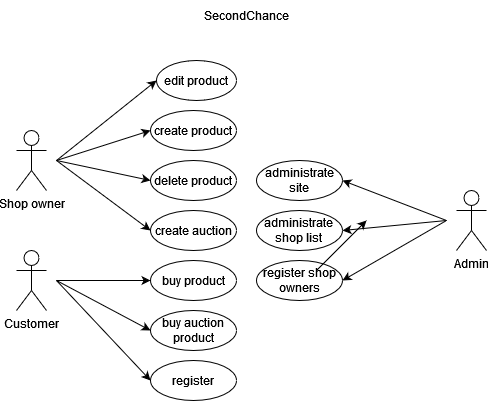
\includegraphics[scale=0.9]{figures/user-case.png}
    \caption{User-case diagram}
    \label{fig:user-case}
\end{figure}
\clearpage


\section{Activity diagram}
The activity diagram describes the actions that are performed on the web-site. Clients should have a registered account to purchase the product. If the client does not have it, he would not be able to buy selected products. Next step is checking if the product is still available or not. If not, the actions will end. When a selected product is available, the next action is payment. Only on condition that the payment goes through, the order is confirmed. If payment does not go through, the process ends without purchasing the product. (See Figure \ref{fig:activity-shop}).

\begin{figure}[h!]
    \centering
    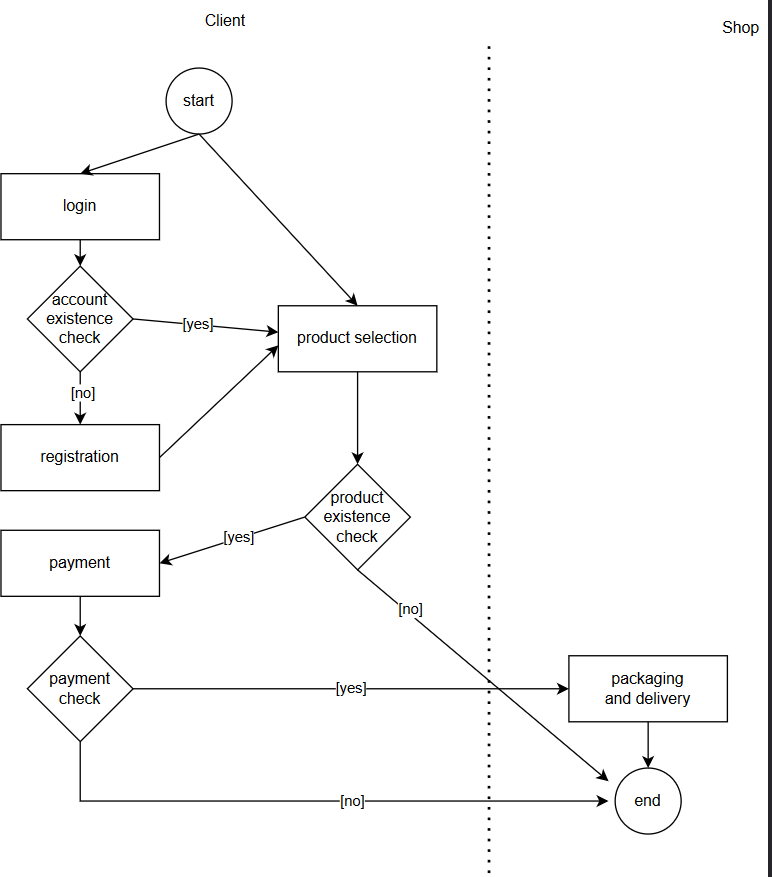
\includegraphics[scale=0.6]{figures/activity-shop.png}
    \caption{Activity-shop diagram}
    \label{fig:activity-shop}
\end{figure}
\clearpage

The last diagram was about the shop system. This one shows the functionality of the auction system. (See Figure \ref{fig:activity-auction}).

\begin{figure}[h!]
    \centering
    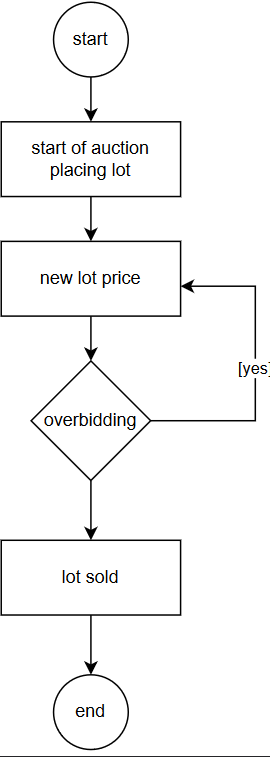
\includegraphics[scale=0.6]{figures/activity-auction.png}
    \caption{Activity-auction diagram}
    \label{fig:activity-auction}
\end{figure}

